%
% IEEE Transactions on Microwave Theory and Techniques example
% Tibault Reveyrand - http://www.microwave.fr
%
% http://www.microwave.fr/LaTeX.html
% ---------------------------------------



% ================================================
% Please HIGHLIGHT the new inputs such like this :
% Text :
%  \hl{comment}
% Aligned Eq. 
% \begin{shaded}
% \end{shaded}
% ================================================



\documentclass[journal]{IEEEtran}

%\usepackage[retainorgcmds]{IEEEtrantools}
%\usepackage{bibentry}  
\usepackage{xcolor,soul,framed} %,caption

\colorlet{shadecolor}{yellow}
% \usepackage{color,soul}
\usepackage[pdftex]{graphicx}
\graphicspath{{../pdf/}{../jpeg/}}
\DeclareGraphicsExtensions{.pdf,.jpeg,.png}

\usepackage[cmex10]{amsmath}
%Mathabx do not work on ScribTex => Removed
%\usepackage{mathabx}
\usepackage{array}
\usepackage{mdwmath}
\usepackage{mdwtab}
\usepackage{eqparbox}
\usepackage{url}

\hyphenation{op-tical net-works semi-conduc-tor}

%\bstctlcite{IEEE:BSTcontrol}


%=== TITLE & AUTHORS ====================================================================
\begin{document}
\bstctlcite{IEEEexample:BSTcontrol}
    \title{LABORATORY NO.~1}
  \author{Manuel Deaza,~\IEEEmembership{Student Member,~ECCI}% <-this % stops a space
  }  


% The paper headers
\markboth{LABORATORY NO.~1, AGUST~2022
}
{Roberg 
\MakeLowercase{\textit{et al.}}: High-Efficiency Diode and Transistor Rectifiers}


% ====================================================================
\maketitle



% === ABSTRACT ====================================================================
% =================================================================================
\begin{abstract}

The next article will present and analyze collected data of first laboratory about pascal laws, in a demonstration with an u-tube and two fluids of different densities, in this case water and oil.
%\boldmath
\end{abstract}


% === KEYWORDS ====================================================================
% =================================================================================
\begin{IEEEkeywords}

\end{IEEEkeywords}






% For peer review papers, you can put extra information on the cover
% page as needed:
% \ifCLASSOPTIONpeerreview
% \begin{center} \bfseries EDICS Category: 3-BBND \end{center}
% \fi
%
% For peerreview papers, this IEEEtran command inserts a page break and
% creates the second title. It will be ignored for other modes.
\IEEEpeerreviewmaketitle


% ====================================================================
% ====================================================================
% ====================================================================











% === I. INTRODUCTION =============================================================
% =================================================================================
\section{Introduction}

Imagina una jeringa con agua, esta misma se encuentra con un tubo plástico de calibre pequeño en la punta de su orificio, al otro lado de este tubo se encuentra una segunda jeringa del mismo modo que la primera, pero esta se encuentra totalmente retraída y sin ningún tipo de fluido dentro. Cuando se le es aplicada una fuerza a la jeringa con agua se ve esta fuerza representada como el desplazamiento del muelle en la otra jeringa sin fluido, la cual empezara a desplazar su muelle saliendo de su camisa, con una fuerza directamente proporcional a la de la jeringa con agua Fig.~\ref{jeringa-example}, esto se relaciona directamente con la ley de Pascal, la cual sera base para el análisis y trabajo que se presentara a continuación.

\begin{figure}[h]
  \begin{center}
  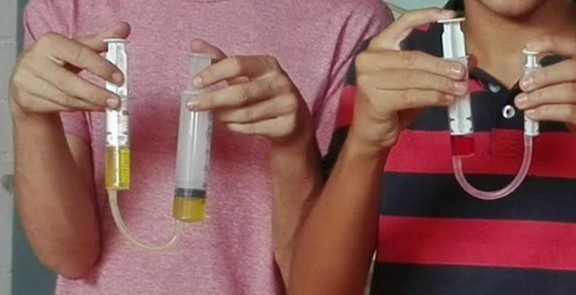
\includegraphics[width=3.3in]{photo/introduccion-example.jpg}\\
  \caption{Representación Ley Pascal con dos jeringas y un tubo, tomado de \cite{pascal-jeringas}}\label{jeringa-example}
  \end{center}
\end{figure}
 
En un primer momento se aterrizara en conceptos sobre la ley de Pascal en relación con el modelo a tratar del famoso "tubo en u" con dos fluidos diferentes en su interior, después de esto se realizara el montaje además de la recolección de las variables fundamentales en este sistema, respectivamente $h$ y $L$.

Por ultimo se realizara una aproximación de datos con la herramienta Python a la ecuación lineal que se presentará, esto se realizo para estimar y comparar los comportamientos con el trabajo que se realizo en la practica.
% === II. Harmonically-Terminated Power Rectifier Analysis ========================
% =================================================================================
\section{State Art}

\subsection{Pascal's law}
\textit{"Debido a las características de los fluidos, es decir, los líquidos, es imposible aplicar presión en algún punto sobre ellos. Para esto, es necesario que la fuerza se ejerza sobre una superficie. Esta fuerza, se expresa como la fuerza por unidad de área, la presión"} \cite{pascal-teory} se puede ver representada como $P = \frac{F}{A}$.

\begin{figure}[h]
  \begin{center}
  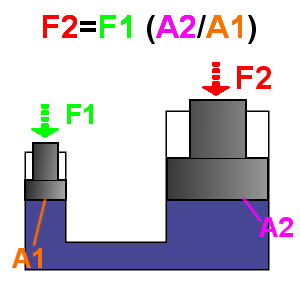
\includegraphics[width=3in]{photo/Hydraulic_Force,_language_neutral.png}\\
  \caption{Representación Ley Pascal como principio de la prensa hidráulica, tomado de \cite{pascal-hidraulica}}\label{law-pascal-example-hidraulica}
  \end{center}
\end{figure}

También se puede llegar a relacionar como el principio de las prensas hidráulicas, un ejemplo se puede ver en Fig.\ref{law-pascal-example-hidraulica} donde la fuerza $F_{1}$ aplicada en una área determinada $A_{1}$ es igual a la fuerza evidenciada en $F_{2}$ en el área $A_{2}$. 
% === III. Schottky-Diode Class-C Rectifier =======================================
% =================================================================================
\section{Objetives}
\subsection{General}
\begin{itemize}
  \item Encontrar la densidad del aceite de oliva con ayuda del principio de pascal.
\end{itemize}

\subsection{Specifics}
 \begin{itemize}
  \item Determinar una expresión que relacione las variables requeridas.
  \item Identificar la relación presente entre cada variable del sistema.
\end{itemize}

% === IV. Transistor Class-F inv Rectifier ========================================
% =================================================================================
\section{Theorical Framework}



Inicialmente se tiene un tubo en forma de U con agua en su interior en reposo, como se ve en la Fig.~\ref{u-tube-master}, posteriormente se le añade una cantidad $L$ de aceite, tomando como referencia la linea punteada que cruza los dos modelos, se logra notar un desplazamiento $h$ de agua.

\begin{figure}[h]
  \begin{center}
  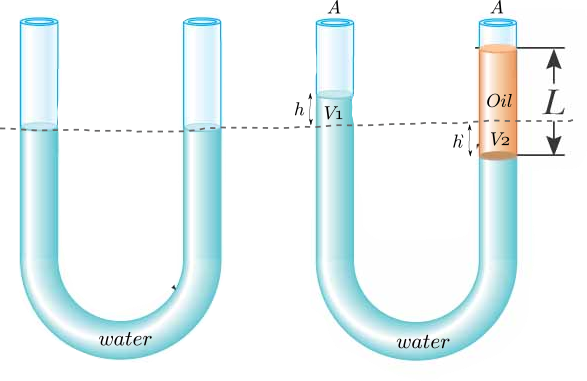
\includegraphics[width=3.7in]{photo/u-tube-example-final.png}\\
  \caption{Representacion grafica tubo en U, a su izquierda el tubo en su estado inicial (solo agua), a su izquierda después de haber introducido el aceite.}\label{u-tube-master}
  \end{center}
\end{figure}

Se puede determinar en base a lo anterior que el volumen desplazado en el brazo izquierdo una vez es introducido el aceite relacionado con $V_2 = hA$,  es igual a $V_1 = h^{\prime}A$ que relaciona el volumen de aceite nuevo debajo de la linea punteada.

Entonces se puede determinar que:
\begin{align*}
V_1 &= V_2 \\
hA  &=  h^{\prime}A 
\end{align*}

Obteniendo una relacion entre $h$ y $h^{\prime}$ denotada por:
\begin{equation}
\label{relacion_aches}
        h = h^{\prime}       
\end{equation}

Ahora con la relacion dada gracias a la ley de pascal que relaciona la presion como la fuerza por una área determinada, asumiendo que la presion ejercida sobre la columna de $Oil$ en el brazo derecho es igual a la del brazo izquierdo, entonces:

\begin{align*}
P_1 &= P_2\\
\frac{F_1}{A} &=  \frac{F_2}{A} 
\end{align*}

Despejando la superficie $A$ donde se ejerce $F_1$ se logra ignorar dicho valor y se obtiene con leyes de newton:

\begin{align*}
F_1 &= F_2\\
m_1g\ &=  m_2g 
\end{align*}

que relacionado con $m = \varrho_{(fluid)}V_{(fluid)}$ donde con valores presentes $V_{(fluid)} = Ah$ y cancelando la gravedad $g$ buscando una relacion proporcional entre $h$ y $L$ se obtiene:

\begin{align*}
\varrho_{(H_{2}O)}Ah &= \varrho_{(Oil)}[L-h]A\\
\end{align*}

Recordando \ref{relacion_aches} se determina que $longitud_{Oil} = [L-h]$, entonces: 

\begin{align*}
\varrho_{(H_{2}O)}Ah &= \varrho_{(Oil)}AL - \varrho_{(Oil)}Ah\\
hA(\varrho_{(H_{2}O)} + \varrho_{(Oil)}) &= \varrho_{(Oil)}AL\\
\end{align*}

para lograr la expresion:

\begin{equation}
\label{h_funcion_L}
h = \frac{\varrho_{(Oil)}}{\varrho_{(H_{2}O)} + \varrho_{(Oil)}} L     
\end{equation}

donde en \ref{h_funcion_L} $h$ es directamente proporcional a $L$ con una pendiente igual a:

\begin{equation}
\label{pendiente_function}
m = \frac{\varrho_{(Oil)}}{\varrho_{(H_{2}O)} + \varrho_{(Oil)}}     
\end{equation}

\section{Laboratory Description}

Inicialmente se tiene un tubo de calibre pequeño con agua en su interior, se quiere insertar paulatinamente aceite por un lado para poder determinar con la variación de $h$ y $L$ la densidad del aceite, en este caso se usara aceite de oliva, el experimento se encuentra montado en el tablero de clase en posición vertical como se ve en Fig.~\ref{u-tube-master-class}.

\begin{figure}[htbp]
  \begin{center}
  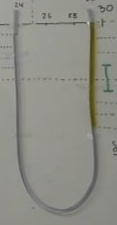
\includegraphics[width=1.8in]{photo/u-tube-class.png}
  \caption{Representación clase tubo-u una vez insertado el aceite, inicialmente se encontraba como en el estado inicial de Fig.~\ref{u-tube-master} pero no se logro obtener un recurso con esa información visual.}\label{u-tube-master-class}
  \end{center}
\end{figure}

\begin{figure}[htbp]
  \begin{center}
  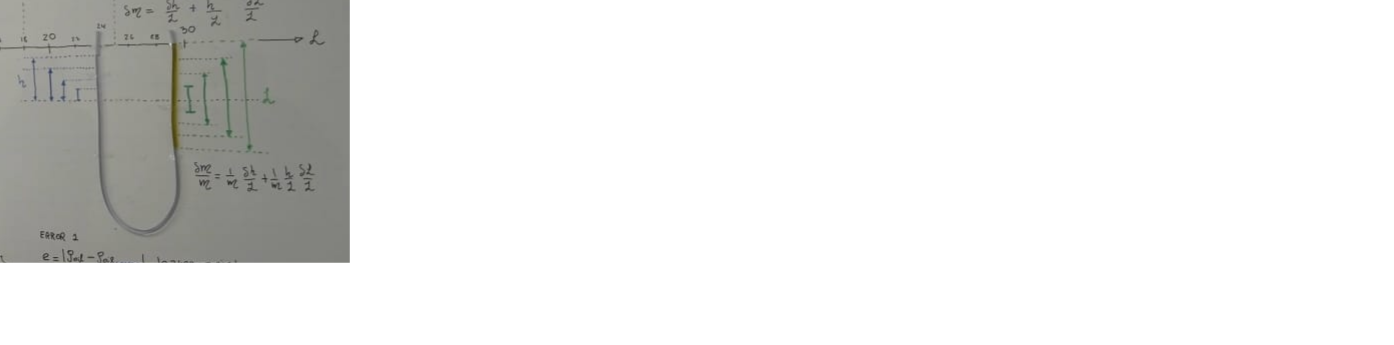
\includegraphics[width=12in]{photo/u-tube-class-marks.png}
  \caption{Representación clase tubo-u una vez insertado el aceite, con las marcas del proceso en busca de la densidad del aceite de oliva. $h$ y $l$ de Fig.~\ref{u-tube-master} }\label{u-tube-master-class-marks}
  \end{center}
\end{figure}

El proceso consiste en inicialmente establecer una posición inicial al tubo junto al agua con una linea punteada de referencia como se observo en Fig.\ref{u-tube-master}, seguido se generaran varias inserciones de aceite de oliva donde en cada una se deberá marcar y medir la distancia que se desplaza el agua determinada por $h$ además de la longitud en la columna de aceite determinada por $L$.  

Posterior se deberá relacionar dichos valores con \ref{h_funcion_L} y \ref{pendiente_function} respectivamente para poder determinar la densidad del aceite de oliva.

El paso a paso se puede evidenciar de una mejor manera en Fig.~\ref{step-by-step-lab} teniendo en cuenta que para la practica se realizaron 5 mediciones.

\begin{figure}[htbp]
  \begin{center}
  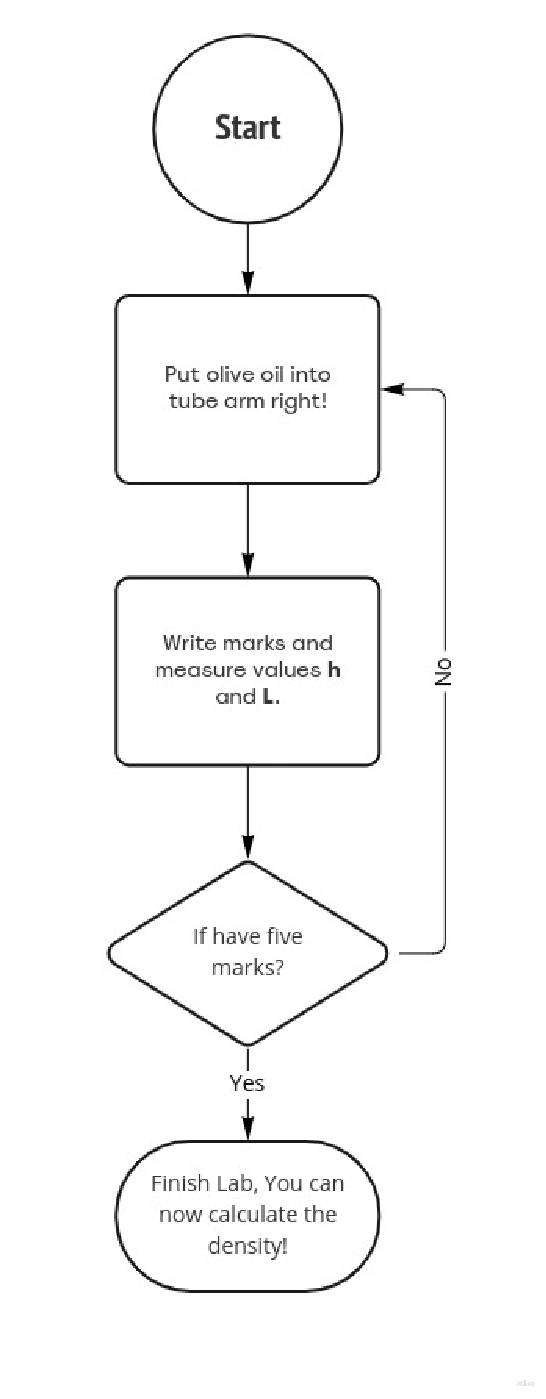
\includegraphics[width=2.3in]{pdf/step_by_step_lab_v2.pdf}
  \caption{Step By Step laboratory, represent in a flowchart.}\label{step-by-step-lab}
  \end{center}
\end{figure}



\section{Results}

\begin{table}[htbp]
\caption{Mediciones de $h$ y $L$}
\begin{center}
\begin{tabular}{|c|c|}
\hline
\textbf{$L_{(cm)}$} & \textbf{$h_{(cm)}$} \\
[0.5ex]\hline\hline
0 & 0\\
\hline
2.7 & 6\\
\hline
4.8 & 12 \\
\hline
8 & 18 \\
\hline
10.6 & 25 \\
\hline
\end{tabular}
\label{tab1}
\end{center}
\end{table}

%Dr. Reveryrand would like to acknowledge the funding by XLIM, Limoges, France. 
Se recolecto los datos en \textbf{5} mediciones de $h$ y $L$ presentados en \ref{tab1} y graficados en Fig.~\ref{measure-data-lab}, para retomar el análisis del inciso IV gracias a \ref{pendiente_function} se puede relacionar esta pendiente como:

\begin{equation}
    \label{pendiente-segunda}
    \frac{h}{L} = m
\end{equation}

donde reconstruyendo la tabla \ref{tab1} se obtiene:

\begin{table}[htbp]
\caption{Mediciones de $h$ y $L$}
\begin{center}
\begin{tabular}{|c|c|c|}
\hline
\textbf{$h_{(cm)}$} & \textbf{$L_{(cm)}$} & \textbf{$m$}\\
[0.5ex]\hline\hline
0 & 0 & 0\\
\hline
2.7 & 6 & 0.45\\
\hline
4.8 & 12 &  0.40\\
\hline
8 & 18  & 0.44\\
\hline
10.6 & 25 & 0.42\\
\hline
 & $m_{\bar{x}}$ & 0.428\\
\hline
\end{tabular}
\label{tab2}
\end{center}
\end{table}

Evidenciando \ref{tab2} se añade un nueva columna la cual posee los valores de pendiente para cada intervalo, ahora determinando el valor promedio de la pendiente $m_{\bar{x}}$ , este se puede relacionar con \ref{pendiente-segunda} para obtener la densidad del aceite, entonces:

\begin{equation}
    \label{densidad_oil}
    \frac{m_{\bar{x}}\rho_{H_{2}O}}{1-m_{\bar{x}}} = \rho_{Oil}
\end{equation}

donde remplazando en \ref{densidad_oil} con los valores $m_{\bar{x}}=0.428$ y $\rho_{H_{2}O} = 1 \frac{gr}{cm^3}$, se obtiene que la densidad del aceite de oliva es:

\begin{align*}
     \rho_{Oil} &= \frac{(0.428)}{(1-0.428)} \frac{gr}{cm^3}\\\\
     &= 0.7482 \frac{gr}{cm^3}\\
\end{align*}

La densidad del aceite de oliva esta definida por $\rho_{Oil} = 0.916 \frac{gr}{cm^3}$ \cite{density-oil} se procede a calcular el porcentaje de error en estos dos datos para determinar la exactitud y precisión de las medidas trabajadas, entonces:

\begin{align*}
    \%_{error} &= \frac{\lvert \rho_{Oil} - \rho_{Oil-google} \rvert}{\rho_{Oil-google}}\\\\
    &= \frac{\lvert 0.748 - 0.916 \rvert}{0.916}\\\\
    &= (0.183)100 = 18.3 \%
\end{align*}

Obteniendo un \% de error de $18.3\%$.

\begin{figure}[htbp]
  \begin{center}
  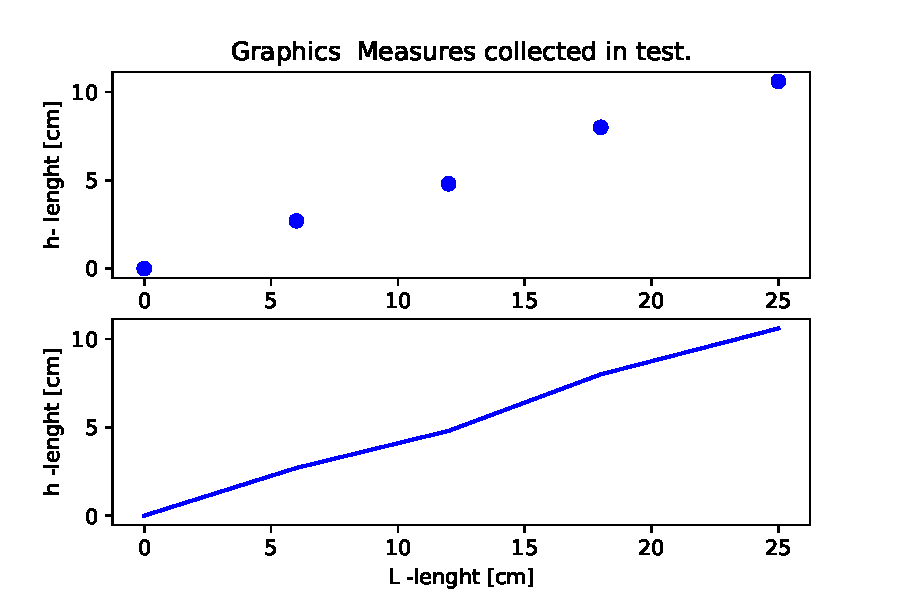
\includegraphics[scale=0.6]{pdf/plot-1-data-collected.pdf}
  \caption{Representacion grafica de Tabla \ref{tab1} }\label{measure-data-lab}
  \end{center}
\end{figure}

Ahora definiendo $L$ como variable independiente y $h$ como variable dependiente se logra relacionar gráficamente dichas variables tomando $m = 0.428$, entonces:

\begin{equation}
\label{equation-time-h}
    h(L) = 0.428L    
\end{equation}

Determinando de esta manera una ecuación lineal que relaciona $h$ y $L$, ahora con ayuda de Python y las librerias Matplotlib, numpy,  se realizo el modelamiento de \ref{equation-time-h} desde una valor inicial $0cm$ hasta $10cm$ en $L$ a un paso de $0.5cm$, como vemos en Fig.~\ref{stimate-system}.

\begin{figure}[htbp]
  \begin{center}
  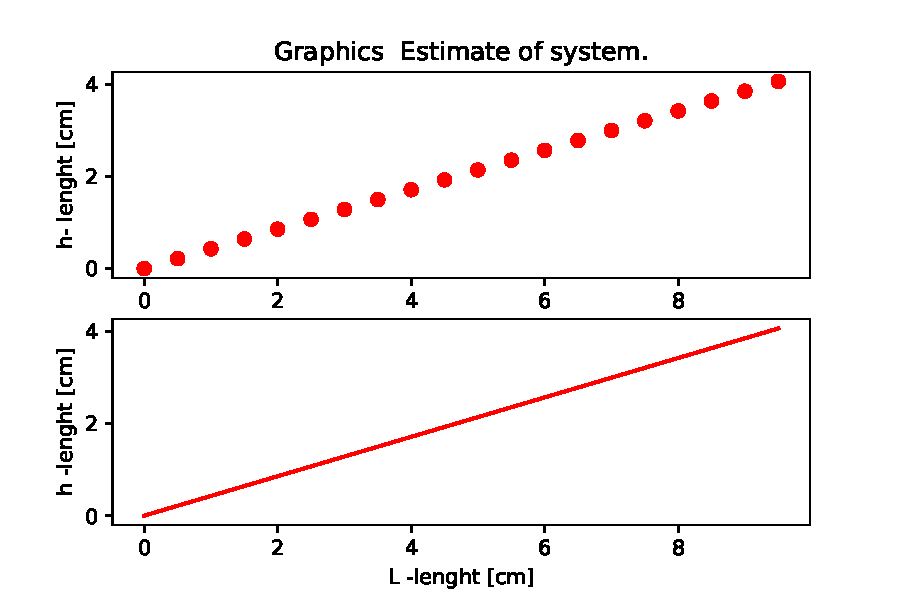
\includegraphics[scale=0.6]{pdf/plot-2-estimate-L.pdf}
  \caption{Estimación de L y h gracias a Python con matplotlib y numpy}\label{stimate-system}
  \end{center}
\end{figure}
    

\section{Conclusions}

Gracias a la ley de Pascal se logro modelar la problemática llegando a un valor de densidad para el aceite de oliva cercano al definido en \cite{density-oil}, esta diferencia es determinada por posible error en medida, ubicación del tubo en el tablero o que el aceite que se uso sea de una menor densidad a la definida en \cite{density-oil}.

A su vez se determina un comportamiento lineal y proporcional entre $h$ y $L$ determinado por \ref{h_funcion_L}, esto se puede validar en Fig.~\ref{measure-data-lab} como también en ecuación que determina el comportamiento en el sistema \ref{equation-time-h}.

En pocas palabras se puede modelar la columna de aceite como un pistón, se establece la relación con el tratamiento que surge del aire en hidráulica con los distintos actuadores, válvulas que vemos en sistemas de este tipo.




% if have a single appendix:
%\appendix[Proof of the Zonklar Equations]
% or
%\appendix  % for no appendix heading
% do not use \section anymore after \appendix, only \section*
% is possibly needed

% use appendices with more than one appendix
% then use \section to start each appendix
% you must declare a \section before using any
% \subsection or using \label (\appendices by itself
% starts a section numbered zero.)
%

% ============================================
%\appendices
%\section{Proof of the First Zonklar Equation}
%Appendix one text goes here %\cite{Roberg2010}.

% you can choose not to have a title for an appendix
% if you want by leaving the argument blank
%\section{}
%Appendix two text goes here.


% use section* for acknowledgement
%\section*{Acknowledgment}


%The authors would like to thank D. Root for the loan of the SWAP. The SWAP that can ONLY be usefull in Boulder...


% Can use something like this to put references on a page
% by themselves when using endfloat and the captionsoff option.
\ifCLASSOPTIONcaptionsoff
  \newpage
\fi



% trigger a \newpage just before the given reference
% number - used to balance the columns on the last page
% adjust value as needed - may need to be readjusted if
% the document is modified later
%\IEEEtriggeratref{8}
% The "triggered" command can be changed if desired:
%\IEEEtriggercmd{\enlargethispage{-5in}}

% ====== REFERENCE SECTION

%\begin{thebibliography}{1}

% IEEEabrv,

\bibliographystyle{IEEEtran}
\bibliography{IEEEabrv, Bibliography}
%\end{thebibliography}
% biography section
% 
% If you have an EPS/PDF photo (graphicx package needed) extra braces are
% needed around the contents of the optional argument to biography to prevent
% the LaTeX parser from getting confused when it sees the complicated
% \includegraphics command within an optional argument. (You could create
% your own custom macro containing the \includegraphics command to make things
% simpler here.)
%\begin{biography}[{\includegraphics[width=1in,height=1.25in,clip,keepaspectratio]{mshell}}]{Michael Shell}
% or if you just want to reserve a space for a photo:

% ==== SWITCH OFF the BIO for submission
% ==== SWITCH OFF the BIO for submission

%% if you will not have a photo at all:
%\begin{IEEEbiographynophoto}{Ignacio Ramos}
%(S'12) received the B.S. degree in electrical engineering from the University of Illinois at Chicago in 2009, and is currently working toward the Ph.D. degree at the University of Colorado at Boulder. From 2009 to 2011, he was with the Power and Electronic Systems Department at Raytheon IDS, Sudbury, MA. His research interests include high-efficiency microwave power amplifiers, microwave DC/DC converters, radar systems, and wireless power transmission.
%\end{IEEEbiographynophoto}

%% insert where needed to balance the two columns on the last page with
%% biographies
%%\newpage

%\begin{IEEEbiographynophoto}{Jane Doe}
%Biography text here.
%\end{IEEEbiographynophoto}
% ==== SWITCH OFF the BIO for submission
% ==== SWITCH OFF the BIO for submission



% You can push biographies down or up by placing
% a \vfill before or after them. The appropriate
% use of \vfill depends on what kind of text is
% on the last page and whether or not the columns
% are being equalized.

\vfill

% Can be used to pull up biographies so that the bottom of the last one
% is flush with the other column.
%\enlargethispage{-5in}



% that's all folks
\end{document}


